\section{Background from Intrinsic Contaminants}
\label{secBackgroundIntrinsic}

Levels of radioactive trace contaminations in xenon might vary at different stages of the experiment, as they strongly depend on purification processes. 
Decays of $^{222}$Rn and $^{85}$Kr in liquid xenon have been simulated with GEANT4 in order to predict  background and to identify the levels of intrinsic contaminants which are tolerable to reach the sensitivity goal of the XENON100 experiment.

In the Monte Carlo simulation, $^{222}$Rn decays have been generated uniformly in the liquid xenon. Only the part of the chain before $^{210}$Pb has been considered, since the relatively long half-life time of 22.3 years for $^{210}$Pb results in radioactive disequilibrium in the decay chain.
The predicted background rate in the energy region below 100~keV is shown in Figure~\ref{figLXeBG_1} as a function of the $^{222}$Rn concentration in the liquid xenon.

\begin{figure}[!h]
\subfigure[]{
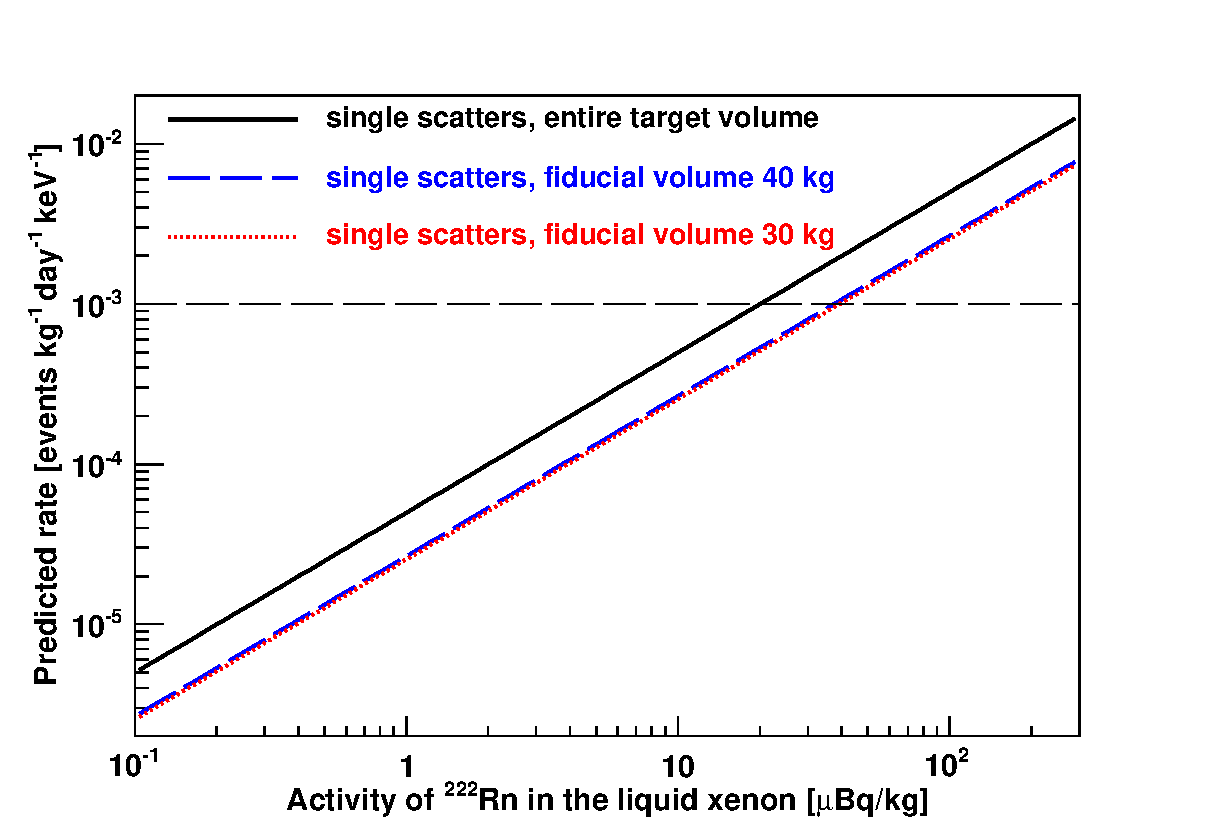
\includegraphics[width=0.475\linewidth]{plots/BackgroundIntrinsic/RnLiquid_Rate-vs-Conc.eps}
\label{figLXeBG_1}}
\subfigure[]{
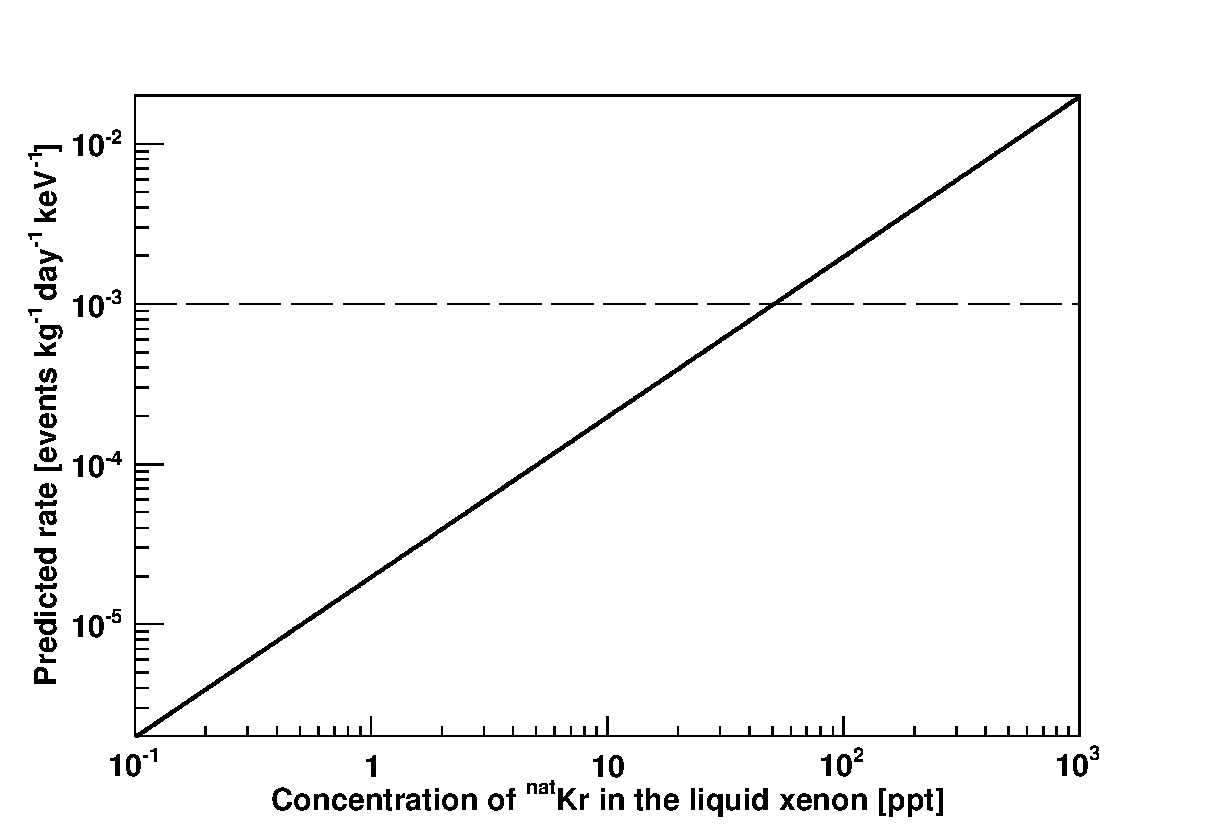
\includegraphics[width=0.475\linewidth]{plots/BackgroundIntrinsic/Kr85_Rate-vs-Conc.eps}
\label{figLXeBG_2}}
\caption[Predicted rate of single electronic recoils with energy below 100~keV for different fiducial masses,  as a function of $^{222}$Rn and $^{\mathrm{nat}}$Kr concentration in the liquid xenon]{
(a) - predicted rate of single electronic recoils with energy below 100~keV for different fiducial masses,  as a function of $^{222}$Rn concentration in the liquid xenon (a).
(b) - predicted background from $^{85}$Kr and a function of $^{\mathrm{nat}}$Kr concentration in the liquid xenon. 
Fiducial and veto cuts are inefficient for this intrinsic background source. As a reference value, the horizontal dashed line corresponds to a background rate of 10$^{-3}$ events$\cdot$kg$^{-1}\cdot$day$^{-1}\cdot$keV$^{-1}$. 
Figures published in Ref.~\cite{EMBG}
}
\label{figLXeBG}
\end{figure}

A background contribution from each intrinsic radioactive source of less than 10$^{-3}$ events$\cdot$kg$^{-1}\cdot$day$^{-1}\cdot$keV$^{-1}$, which is used as a reference value, translates into a concentration of $^{nat}$Kr below 50~ppt, and a $^{222}$Rn activity in the liquid xenon of $<$20~$\mu$Bq/kg in the entire target mass of 62~kg. The background from $^{222}$Rn daughters can be reduced by a fiducial volume cut, removing decays at the edge of the target volume which are likely to produce high energy gamma rays with a longer mean free path, escaping the target volume while generating a single scatter signature. For the 40~kg and 30~kg fiducial volumes, a background level of 10$^{-3}$ events$\cdot$kg$^{-1}\cdot$day$^{-1}\cdot$keV$^{-1}$ corresponds to 35 $\mu$Bq/kg.

The background rate from $^{85}$Kr has been predicted for different  concentrations of $^{\mathrm{nat}}$Kr in the liquid xenon target, and is shown in Figure~\ref{figLXeBG_2}. It consists almost entirely (with an exception of the channel with 0.434\% branching ratio used for delayed coincidence analysis) of electrons with a very short mean free path, thus fiducial volume and veto coincidence cuts are inefficient for background reduction. A background level of 10$^{-3}$ events$\cdot$kg$^{-1}\cdot$day$^{-1}\cdot$keV$^{-1}$ corresponds to a natural krypton concentration of 50~ppt. 
